\subsection{Bifurcação}

A família quadrática exibe outro fenômeno que ocorre em sistemas dinâmicos: a bifurcação.
Através desse fenômeno, vamos explicar gráfica e intuitivamente como a dinâmica de $h$, que é simples para $\mu$ pequeno, se torna caótica para $\mu$ suficientemente grande.

Seja $f_\lambda$ uma família parametrizada de funções no parâmetro $\lambda$ de modo que a função
$$G(x, \lambda) = f_\lambda(x),$$
definida num aberto de $\RR^2$, seja de classe $\class^\infty$ nas variáveis $x$ e $\lambda$.
Dizemos que $f_\lambda$ sofre uma bifurcação em $\lambda_0$ se existe $\varepsilon > 0$ com a seguinte propriedade: se $\lambda_1 \in (\lambda_0 - \varepsilon, \lambda_0)$ e $\lambda_2 \in (\lambda_0, \lambda_0 + \varepsilon)$, então $f_{\lambda_1}$ e $f_{\lambda_2}$ não são topologicamente conjugadas.
Por exemplo, uma bifurcação ocorre quando há alteração na estrutura dos pontos periódicos.

\begin{example}
\begin{enumerate}[label=\alph*)]\item[]
\item 
A família $E_\lambda$ de funções dadas por $E_\lambda(x) = e^{x + \lambda}$ sofre uma bifurcação em $\lambda_0 = -1$.

Conforme o parâmetro cresce, os dois pontos fixos vão se aproximando até se tornarem um único ponto fixo que, após isso, desaparece. Uma bifurcação com essas características é chamada de bifurcação tangente. Ver Figura \ref{fig e_lambda}.

\begin{figure}[!htb]
\label{fig e_lambda}
\centering
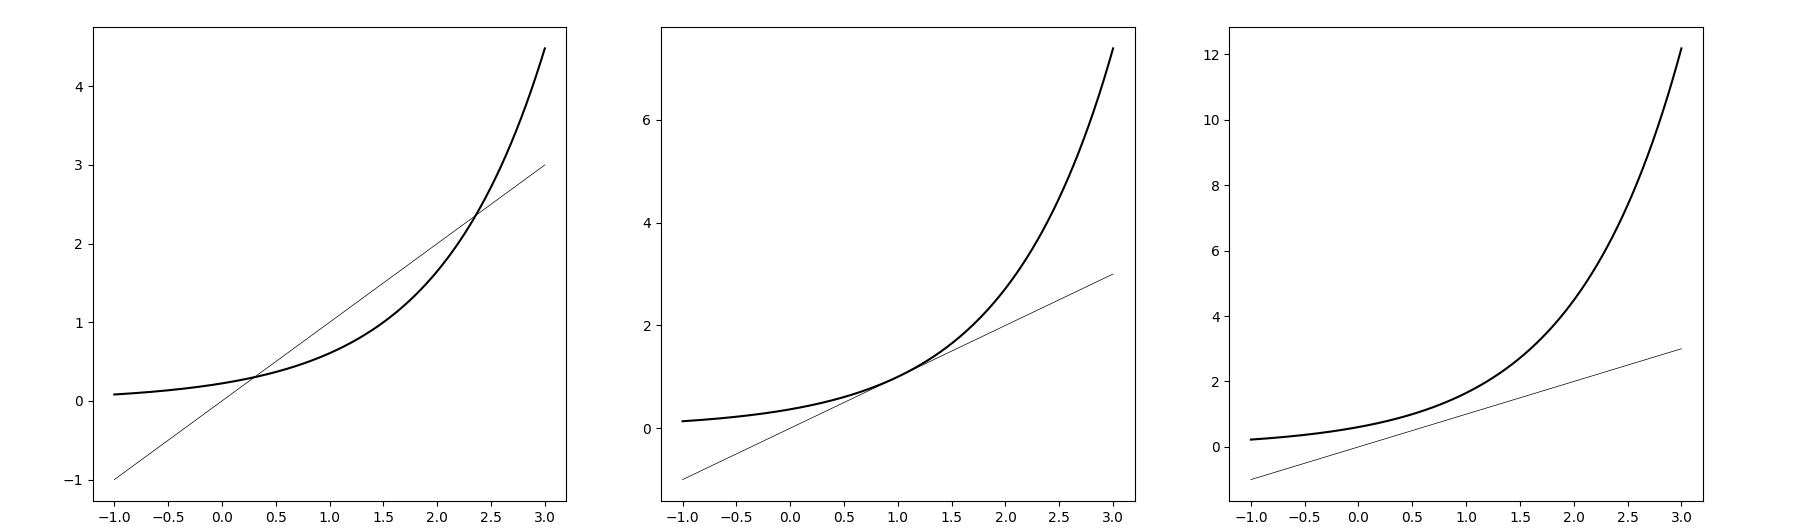
\includegraphics[scale=0.25]{images/e_lambda.png}
\caption{O gráfico de $E_\lambda$ para $\lambda = -1.5$, $\lambda = -1$ e $\lambda = -0.5$, respectivamente.}
\end{figure}

\item A família quadrática sofre uma bifurcação em $\mu_0 = 3$.

Conforme o parâmetro cresce, o ponto fixo, que inicialmente é atrator, se torna repulsor e, além disso, nasce uma órbita periódica de período $2$ numa vizinhança do ponto fixo. Uma bifurcação com essas características é chamada de bifurcação com duplicação de período. Ver Figura \ref{fig h_mu^2}.

\begin{figure}[!htb]
\label{fig h_mu^2}
\centering
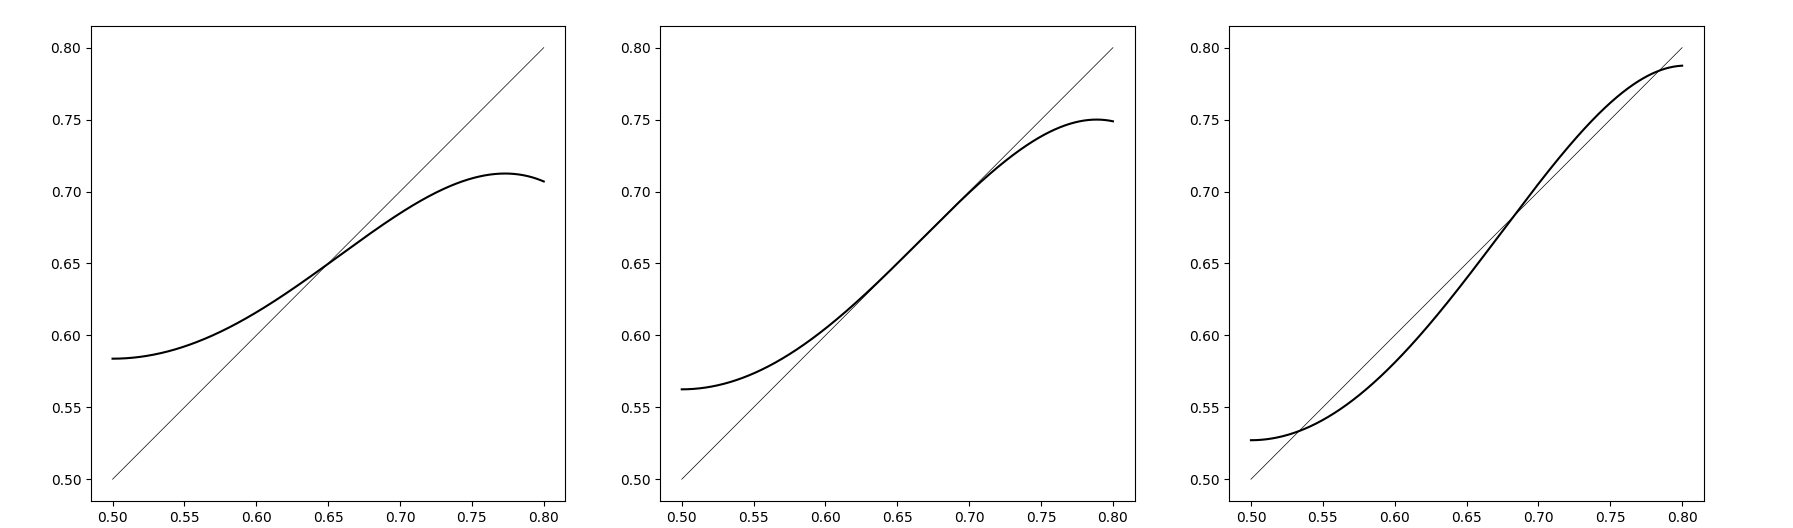
\includegraphics[scale=0.3]{images/h_mu^2.png}
\caption{O gráfico de $h^2$ numa vizinhança de $p_\mu$ para $\mu = 2.85$, $\mu = 3$ e $\mu = 3.15$, respectivamente.}
\end{figure}

\end{enumerate}
\end{example}

Observe, nos exemplos, que as bifurcações ocorreram quando a derivada em módulo no ponto fixo se tornou igual à $1$. O teorema a seguir nos mostra que isso não é coincidência.

\begin{theorem}
\label{theorem1}
Seja $f_\lambda$ uma família parametrizada de funções.
Suponha que
\begin{enumerate}
\item $f_{\lambda_0}(x_0) = x_0$,
\item $f'_{\lambda_0}(x_0) \neq 1$. 
\end{enumerate}
Então existem vizinhanças $I$ e $J$ de $\lambda_0$ e $x_0$, respectivamente, e uma função $p: I \to J$ de classe $\class^\infty$ tais que
\begin{enumerate}
\item $p(\lambda_0) = x_0$, 
\item $f_\lambda(p(\lambda)) = p(\lambda)$ para todo $\lambda \in I$.
\end{enumerate}
Além disso, $f_\lambda$ não possui outros pontos fixos em $J$.
\end{theorem}

\begin{proof}
Basta aplicar o Teorema da Função Implícita para a função $G(x, \lambda) = f_\lambda(x) - x$ no ponto $(x_0, \lambda_0)$.
\end{proof}

Vamos estudar com um pouco mais de detalhes a bifurcação com duplicação de período que ocorre na família quadrática.
Inicialmente, observe que se $\mu > 2$, então existe $p_\mu' < p_\mu$ tal que $h(p_\mu') = p_\mu$.
Na Figura \ref{fig renormalization}, observe o gráfico de $h^2$ para alguns valores de $\mu$, juntamente com um quadrado de vértices $(p_\mu', p_\mu)$, $(p_\mu, p_\mu)$, $(p_\mu, p_\mu')$ e $(p_\mu', p_\mu')$.

\begin{figure}[!htb]
\label{fig h^2-and-boxes}
\centering
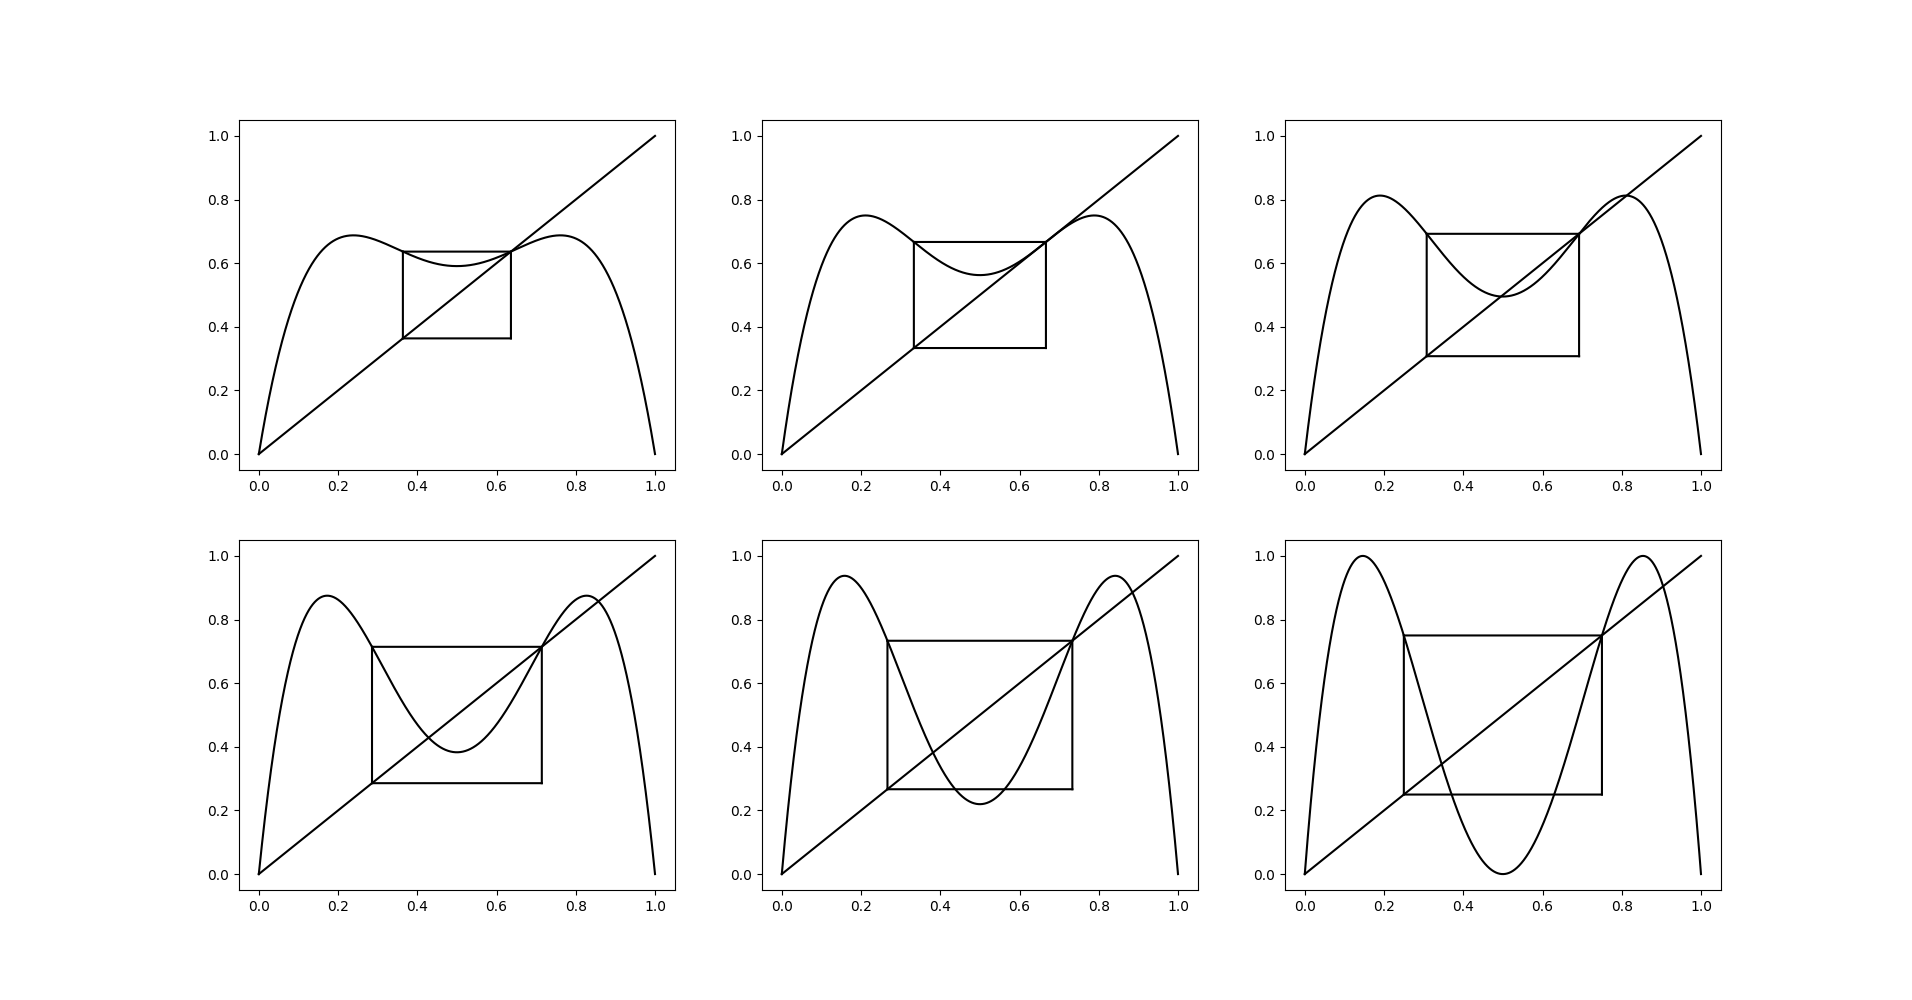
\includegraphics[scale=0.25]{images/h^2-and-boxes.png}
\caption{O gráfico de $h^2$ para $\mu = 2.75$, $\mu = 3$, $\mu = 3.25$, $\mu = 3.5$, $\mu = 3.75$ e $\mu = 4$, respectivamente.}
\end{figure}

Restringindo o gráfico de $h^2$ ao quadrado e rotacionando em $\pi$ radianos, vemos que ele se assemelha ao gráfico da própria $h$ no intervalo $[0, 1]$ para um valor de $\mu$ diferente. Vamos deixar essa ideia mais precisa através do operador de renormalização, que nos permite analisar a segunda iterada de uma função na mesma escala que a original.

Se $\mu > 2$, considere a função $L: [p_\mu', p_\mu] \to [0, 1]$ linear bijetora tal que $L(p_\mu') = 1$ e $L(p_\mu) = 0$.
Desse modo, definimos a renormalização de $h$ como a função $Rh: [0, 1] \to [0, 1]$ dada por $Rh(x) = L \circ h^2 \circ L^{-1}(x)$.
Observe que cada ponto fixo de $Rh$ está relacionado com um ponto periódico de $h$ de período $2$. Além disso, o gráfico de $Rh$ não está contido em $[0, 1]$ para algum $\mu < 4$. Ver Figura \ref{fig renormalization}.

\begin{figure}[!htb]
\label{fig renormalization}
\centering
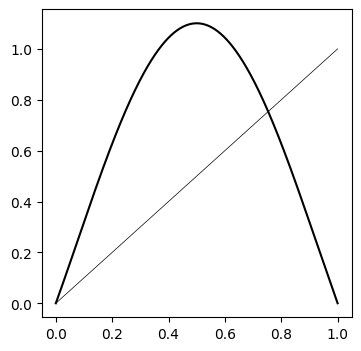
\includegraphics[scale=0.25]{images/renormalization.png}
\caption{Os gráficos de $h^2$ e $Rh$, respectivamente, para $\mu = 3.7$.}
\end{figure}

Desse modo, esperamos que $Rh$ sofra uma bifurcação com duplicação de período conforme o parâmetro cresce e, de maneira análoga, que $h^2$ sofra uma bifurcação com duplicação de período. Continuando esse processo, temos uma sucessão de bifurcações com duplicação de período na família quadrática.

O computador nos permite observar esse fato experimentalmente.
Para isso, vamos computar o digrama de órbita do ponto crítico da família quadrática para $\mu > 2$.
Nesse diagrama, veremos o comportamento assintótico de órbita de $\frac{1}{2}$ em função de $\mu$.
Escolhemos a órbita de $\frac{1}{2}$ para desenhar o diagrama pois, como veremos no Teorema de Singer, se $h$ possui uma órbita periódica atratora, então essa órbita  atrai o ponto crítico.

Para construir o diagrama de órbita, escolhemos $20000$ valores de $\mu$ igualmente espaçados em $[2, 4]$ e, para cada um desses valores, plotamos $h^k(\frac{1}{2})$ na abscissa $\mu$ para todo $200 \leq k \leq 500$.

\begin{figure}[!htb]
\label{fig period-doubling}
\centering
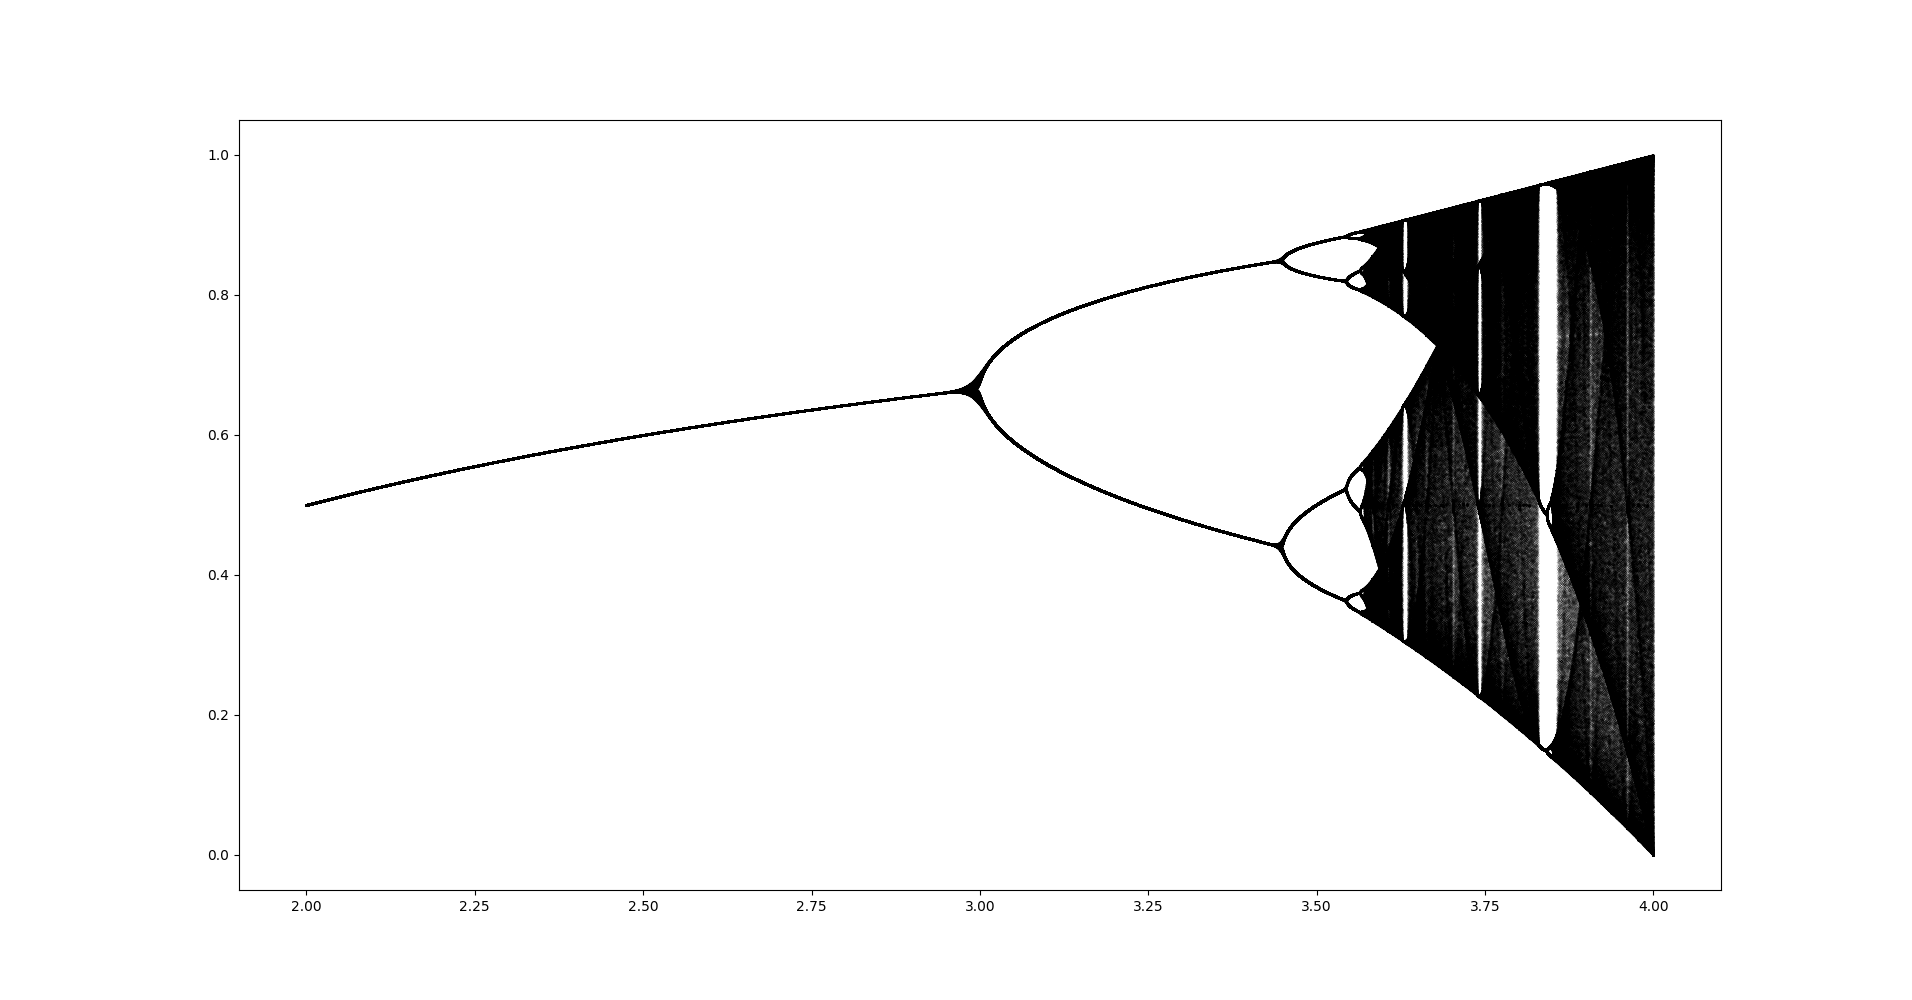
\includegraphics[scale=0.25]{images/period-doubling.png}
\caption{O diagrama de bifurcação de $h$ para $2 \leq \mu \leq 4$.}
\end{figure}

\begin{figure}[!htb]
\label{fig period-doubling1}
\centering
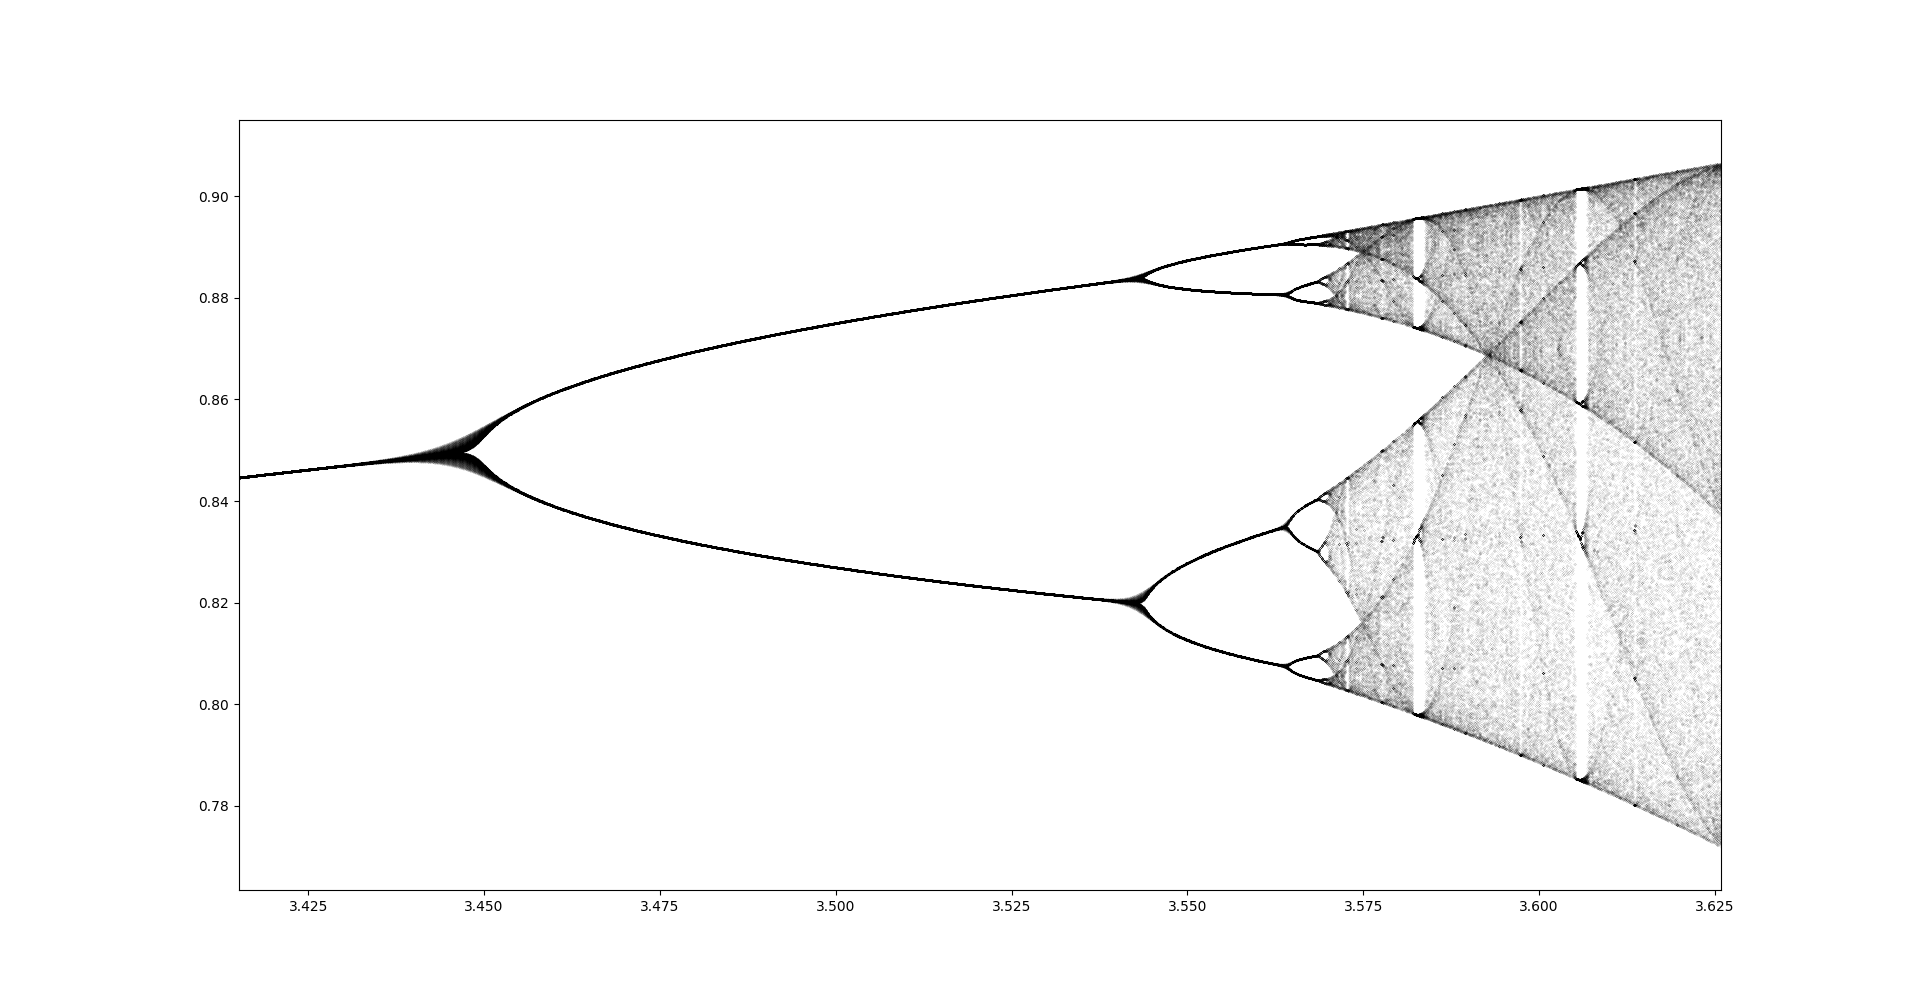
\includegraphics[scale=0.25]{images/period-doubling1.png}
\caption{Uma ampliação no diagrama de bifurcação de $h$.}
\end{figure}

Na Figura \ref{fig period-doubling} vemos alguns fatos que já estudamos: se $\mu \in [2, 3]$, então as órbitas são atraídas para o ponto fixo $p_\mu$; quando $\mu$ passa de $3$, nasce uma órbita periódica de período $2$; e se $\mu = 3.839$, então existe uma órbita atratora de período $3$. 
